\documentclass[pdf]{beamer}
\usepackage{lmodern}
\mode<presentation>{\usetheme{PaloAlto}}
\title{Speckle Interferometry}
\author{Matt Rauen and David Fan}
\date{\today}
\begin{document}
\begin{frame}
\titlepage
\end{frame}

\section{Abstract}
\begin{frame}{Abstract}

\end{frame}

\section{Research Questions}
\begin{frame}{Research Questions}
\begin{center}
Primary Question:

How does the piezo deform when a voltage is applied to it?
\end{center}
More concretely, we want to construct a topological map of the shift at each point, where each point is characterized by the phase difference (relative to the wavelength of light we used) between its original position and its position after the applied voltage.
\begin{figure}[htbp]
\centering
\includegraphics[width=0.3\textwidth]{gaussian_bump.png}
\end{figure}
\end{frame}

\section{Background}
\begin{frame}{Speckle Patterns}
Speckle patterns are generated by interference of a set of wavefronts. In particular, in our experiment, this interference is between light reflected off of the reference object and the object of interest.\\
\vspace{0.5cm}
{\bf Important Property of Speckle Patterns:}
The size of the speckles is inversely proportional to the size of the aperture.
\begin{figure}[!htb]
\minipage{0.3\textwidth}
  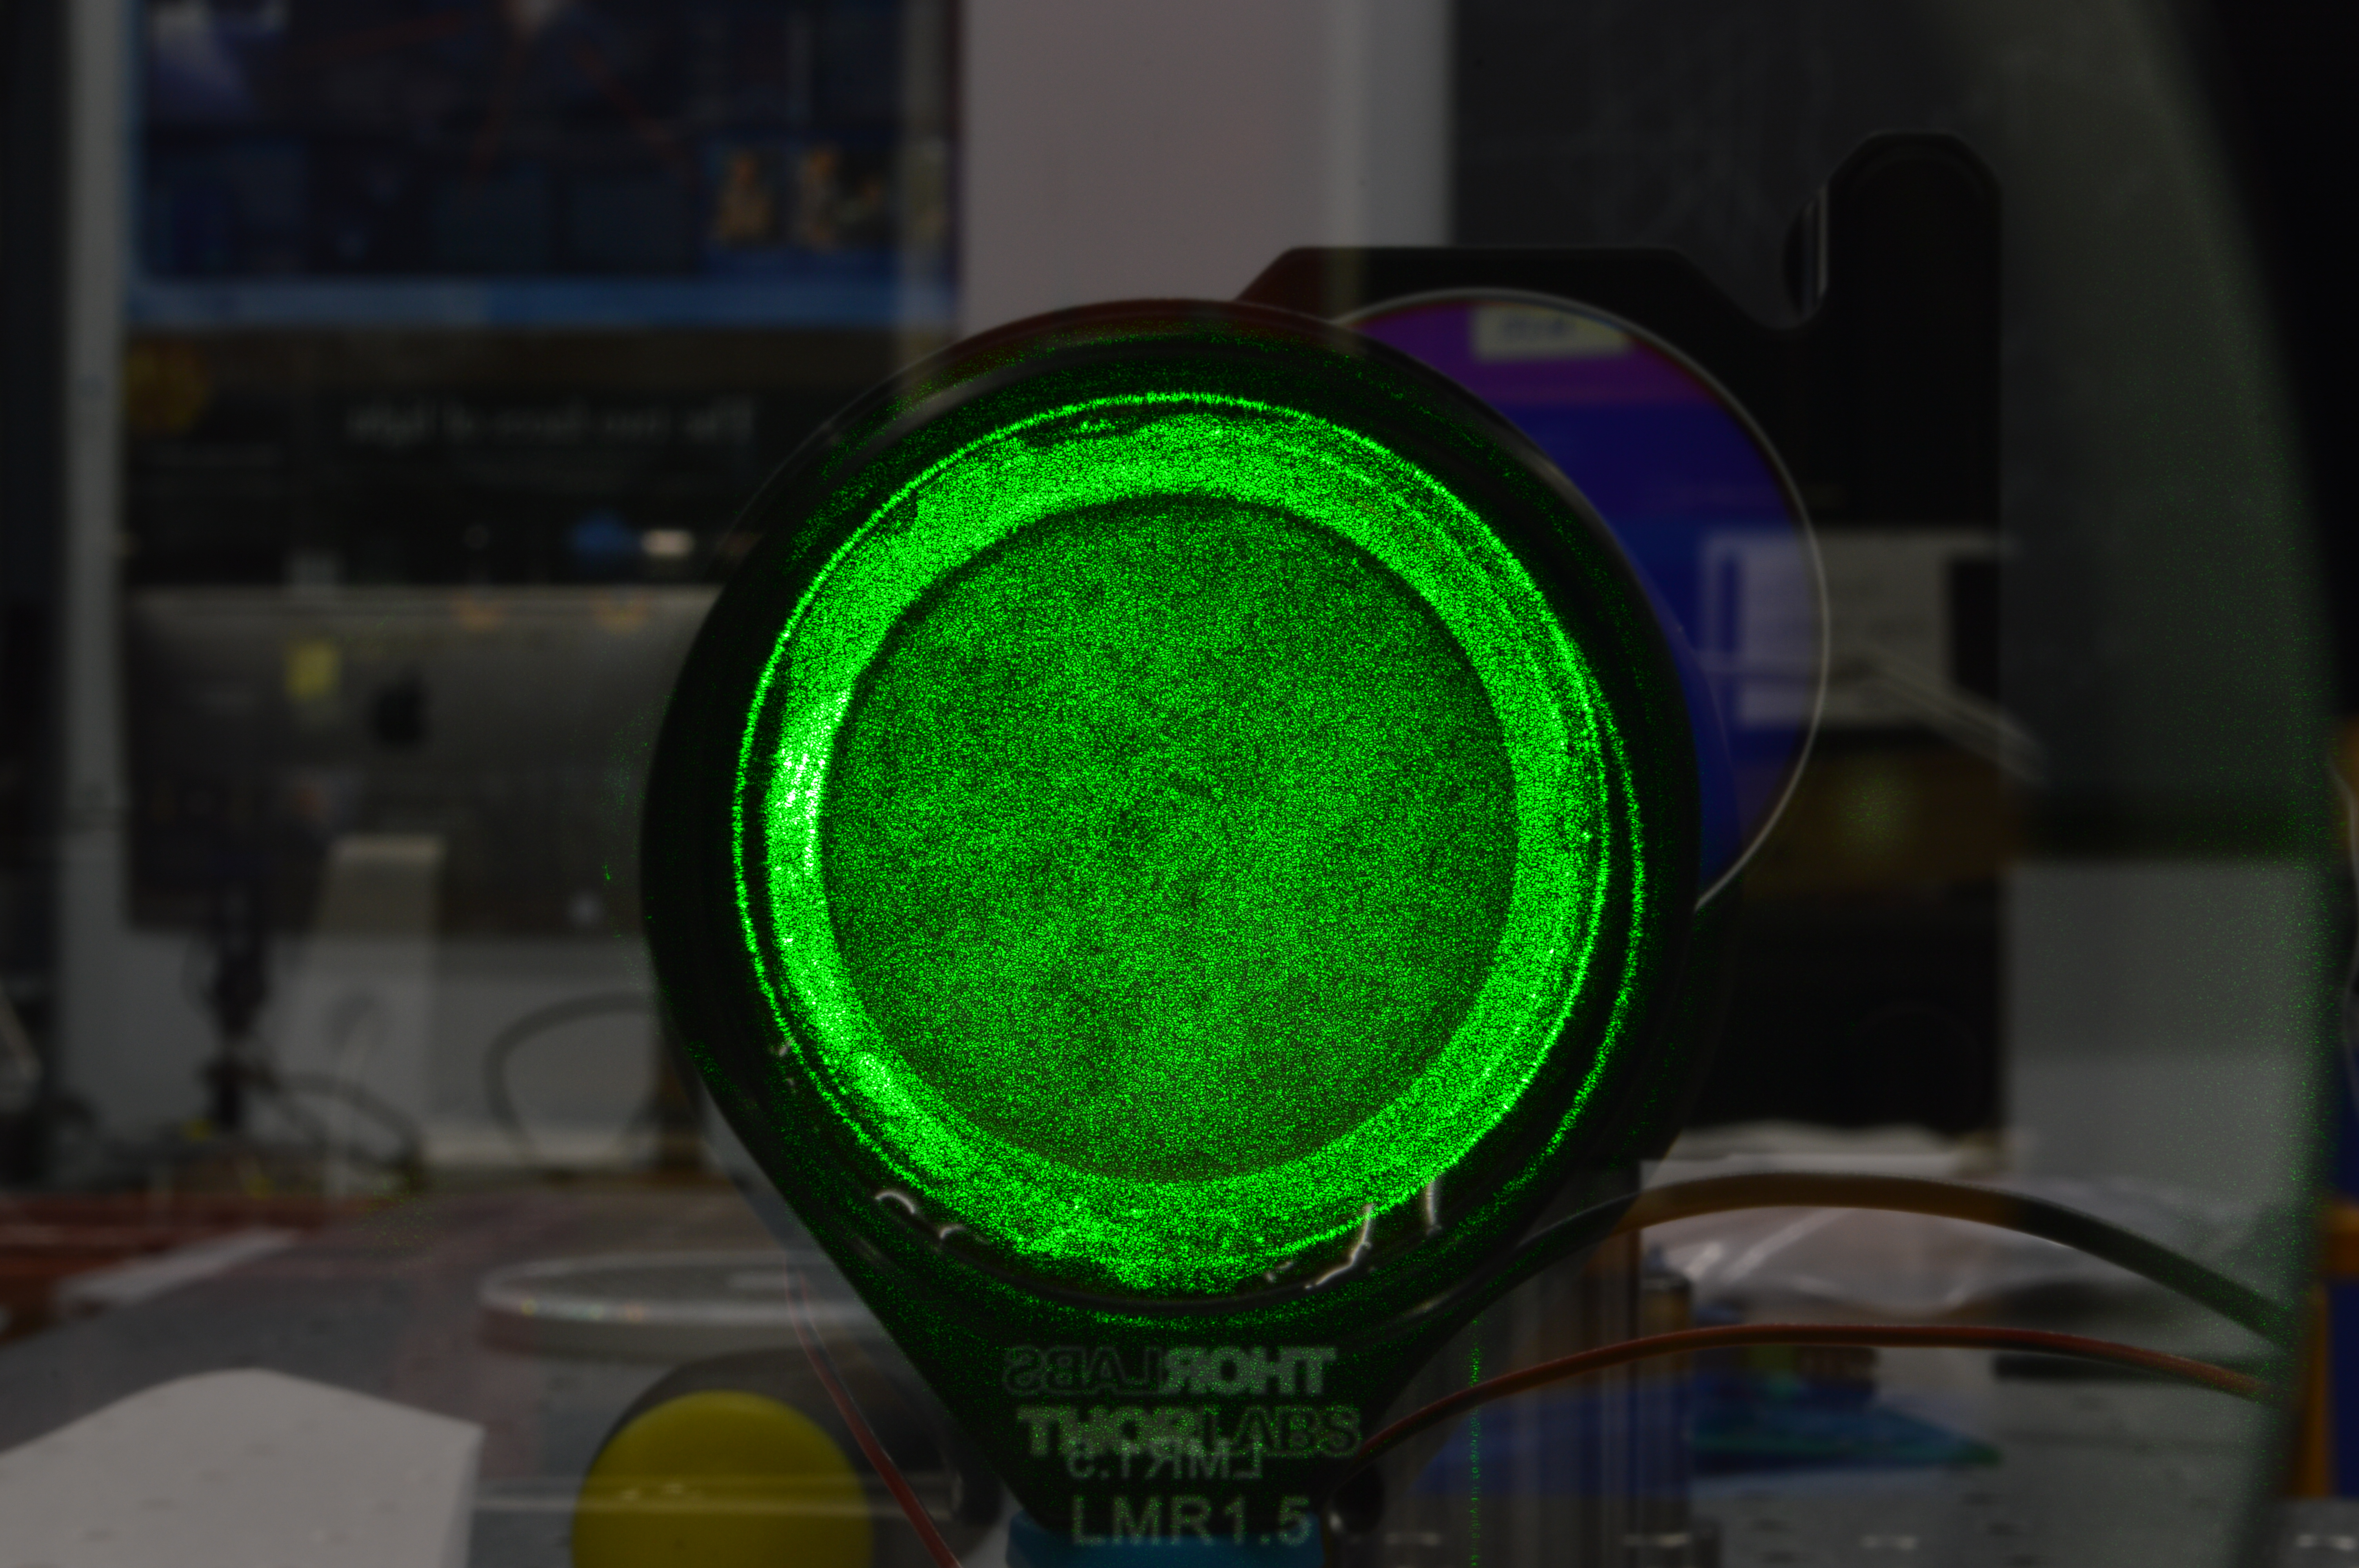
\includegraphics[width=\linewidth]{apertures/32.png}
  \caption{$a=32$}
\endminipage\hfill
\minipage{0.3\textwidth}
  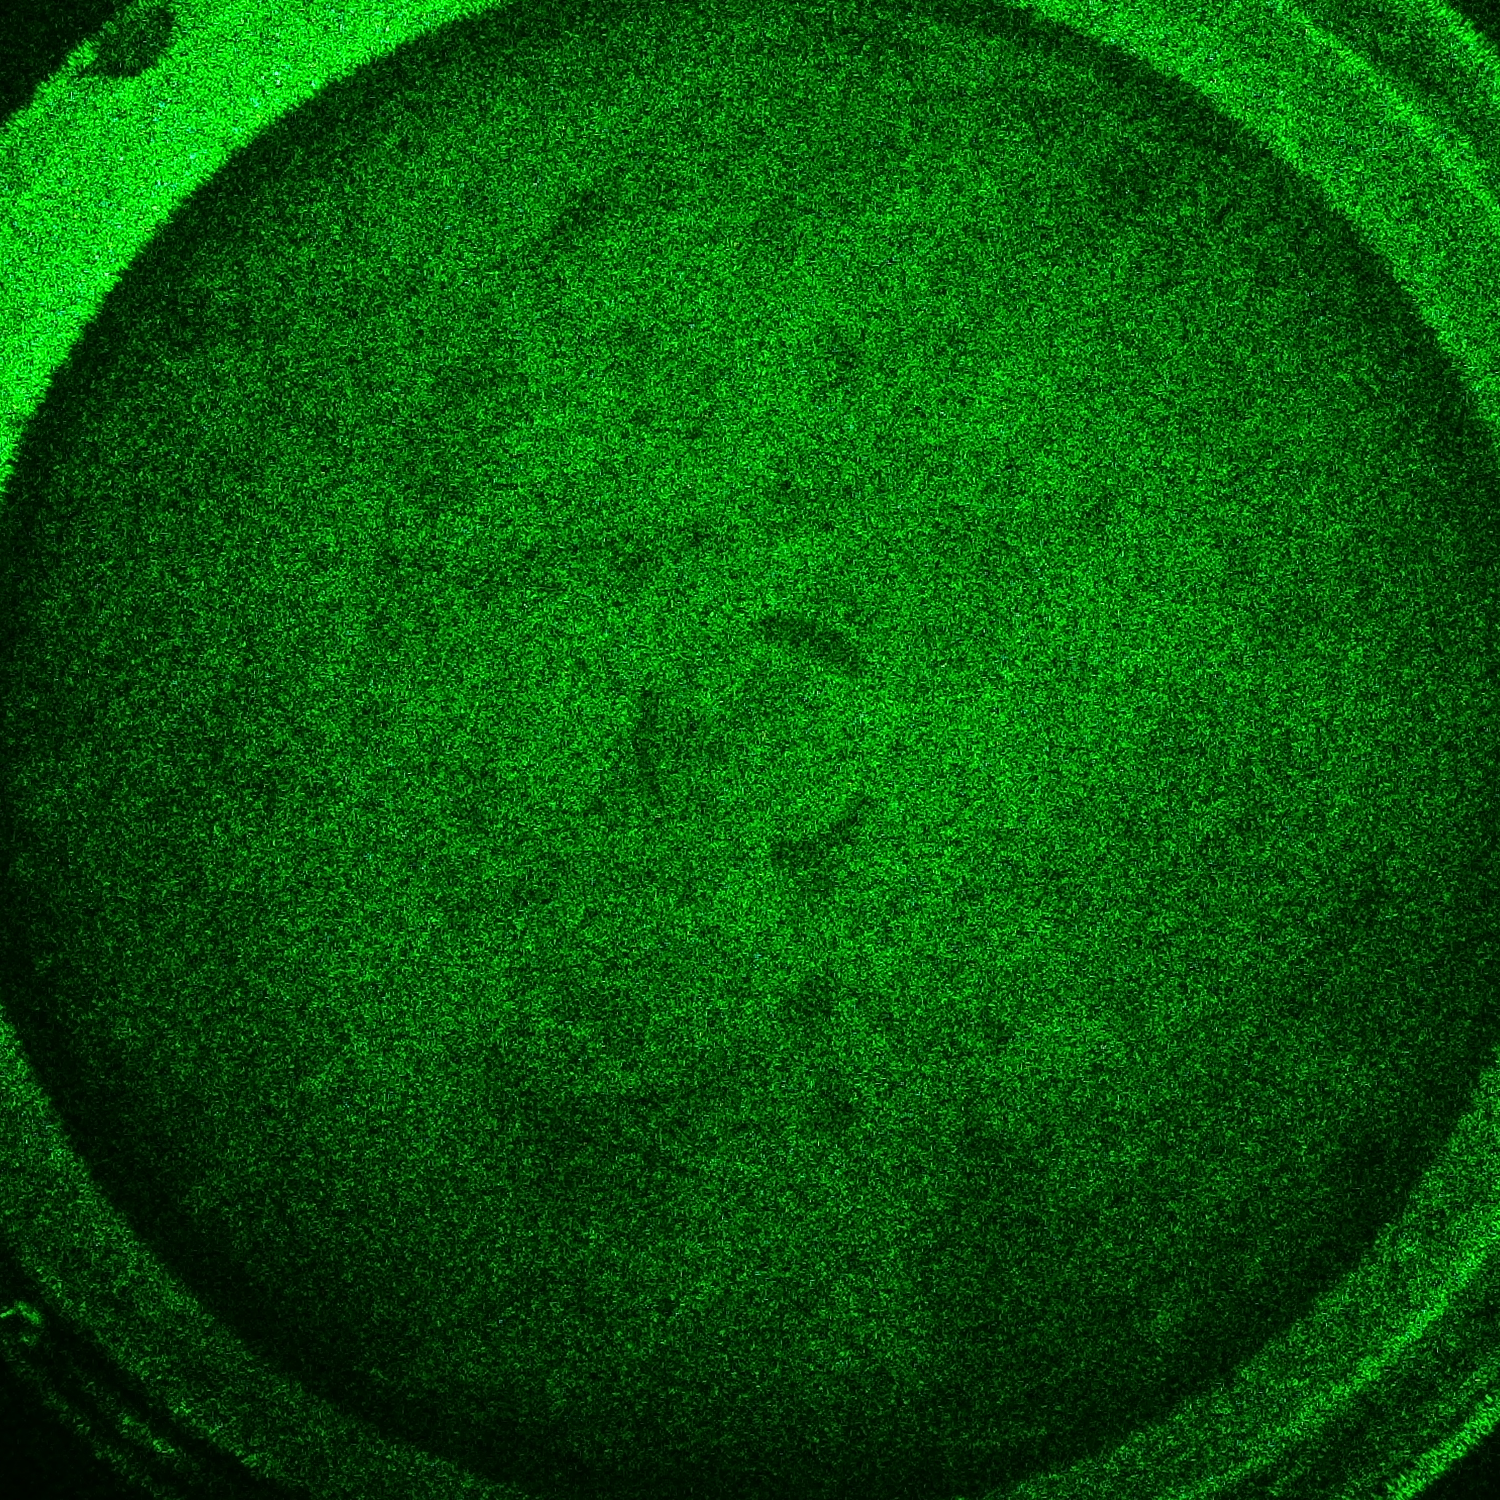
\includegraphics[width=\linewidth]{apertures/16.png}
  \caption{$a=16$}
\endminipage\hfill
\minipage{0.3\textwidth}
  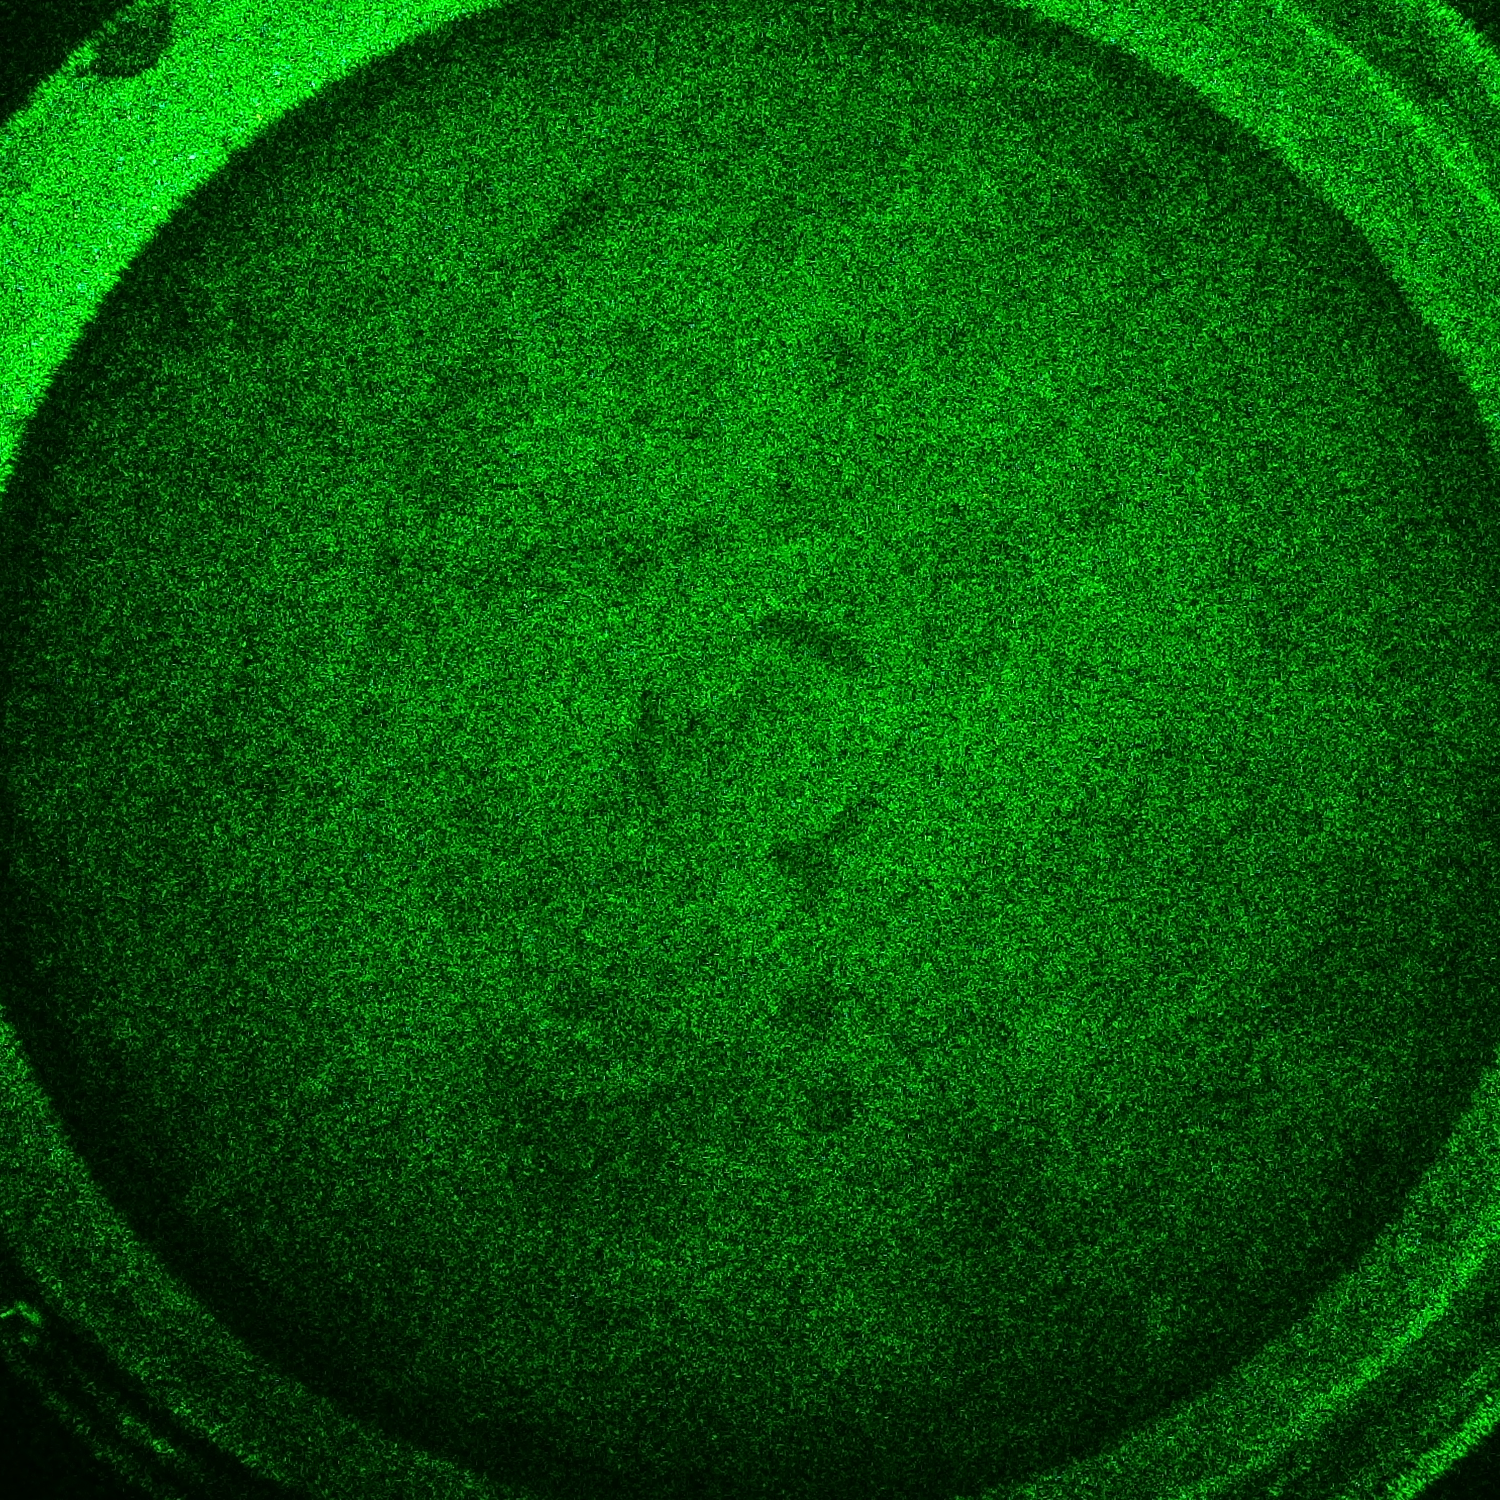
\includegraphics[width=\linewidth]{apertures/5.png}
  \caption{$a=5.6$}
\endminipage
\end{figure}
\end{frame}

\begin{frame}{Modeling Each Speckle}
We can model the intensity of each pixel via the equation$$A\cos x + b_0,$$where $A$ and $b_0$ are fixed constants, and $x$ is proportional to the distance between the aperture and the piezo at that pixel.\\
\vspace{0.5cm}
Therefore, if we translate the reference object, while holding the object of interest stationary, we would expect that the intensities of any given pixel trace out a cosine curve with some offset.
\end{frame}

\section{Setup}
\begin{frame}{Setup}

\end{frame}

\section{Analysis}
\begin{frame}{Calculating Absolute Phases}
If we assume that we have images where the phases have shifted by exactly $\frac13$ of a wavelength, we find the phase of the wave for each pixel by taking the following differences
\begin{align*}
	A\sin(x) &= \frac{pixel3 - pixel2}{\sqrt 3}\\
	A\cos(x) &= -\frac23 \left(\frac{pixel3 + pixel2}{2} - pixel1\right)
\end{align*}
%Note that $b_0$ disappears when taking these differences. 
From this point $A$ is just
$$A = \sqrt{[A\sin(x)]^2 + [A\cos(x)]^2}$$
From this we can find the phase
$$x = \cos^{-1}\left(\frac{A\cos(x)}{A}\right)$$
% if math.sin(guess) * Asinx < 0:
% guess = -guess
\end{frame}

\begin{frame}{Calculating Absolute Phases}
In order to sample at exactly $\frac13$ of a wavelength, we needed to determine how the reference piezo responds to voltage.

\vspace{.5cm}
The interference patterns are periodic, they will repeat their patterns after the reference object has moved by exactly $\frac12$ a wavelength. We did this by manual adjusting the voltage until the same pattern was seen, and recording the voltage.

\vspace{.5cm}
We found that 0.95 to 1.0 volts corresponded to a shift of half a wavelength in the reference piezo (a one wavelength shift in the phase of the the light from the reference piezo)
% \begin{center}
% {\bf One wavelength shift}\\
% 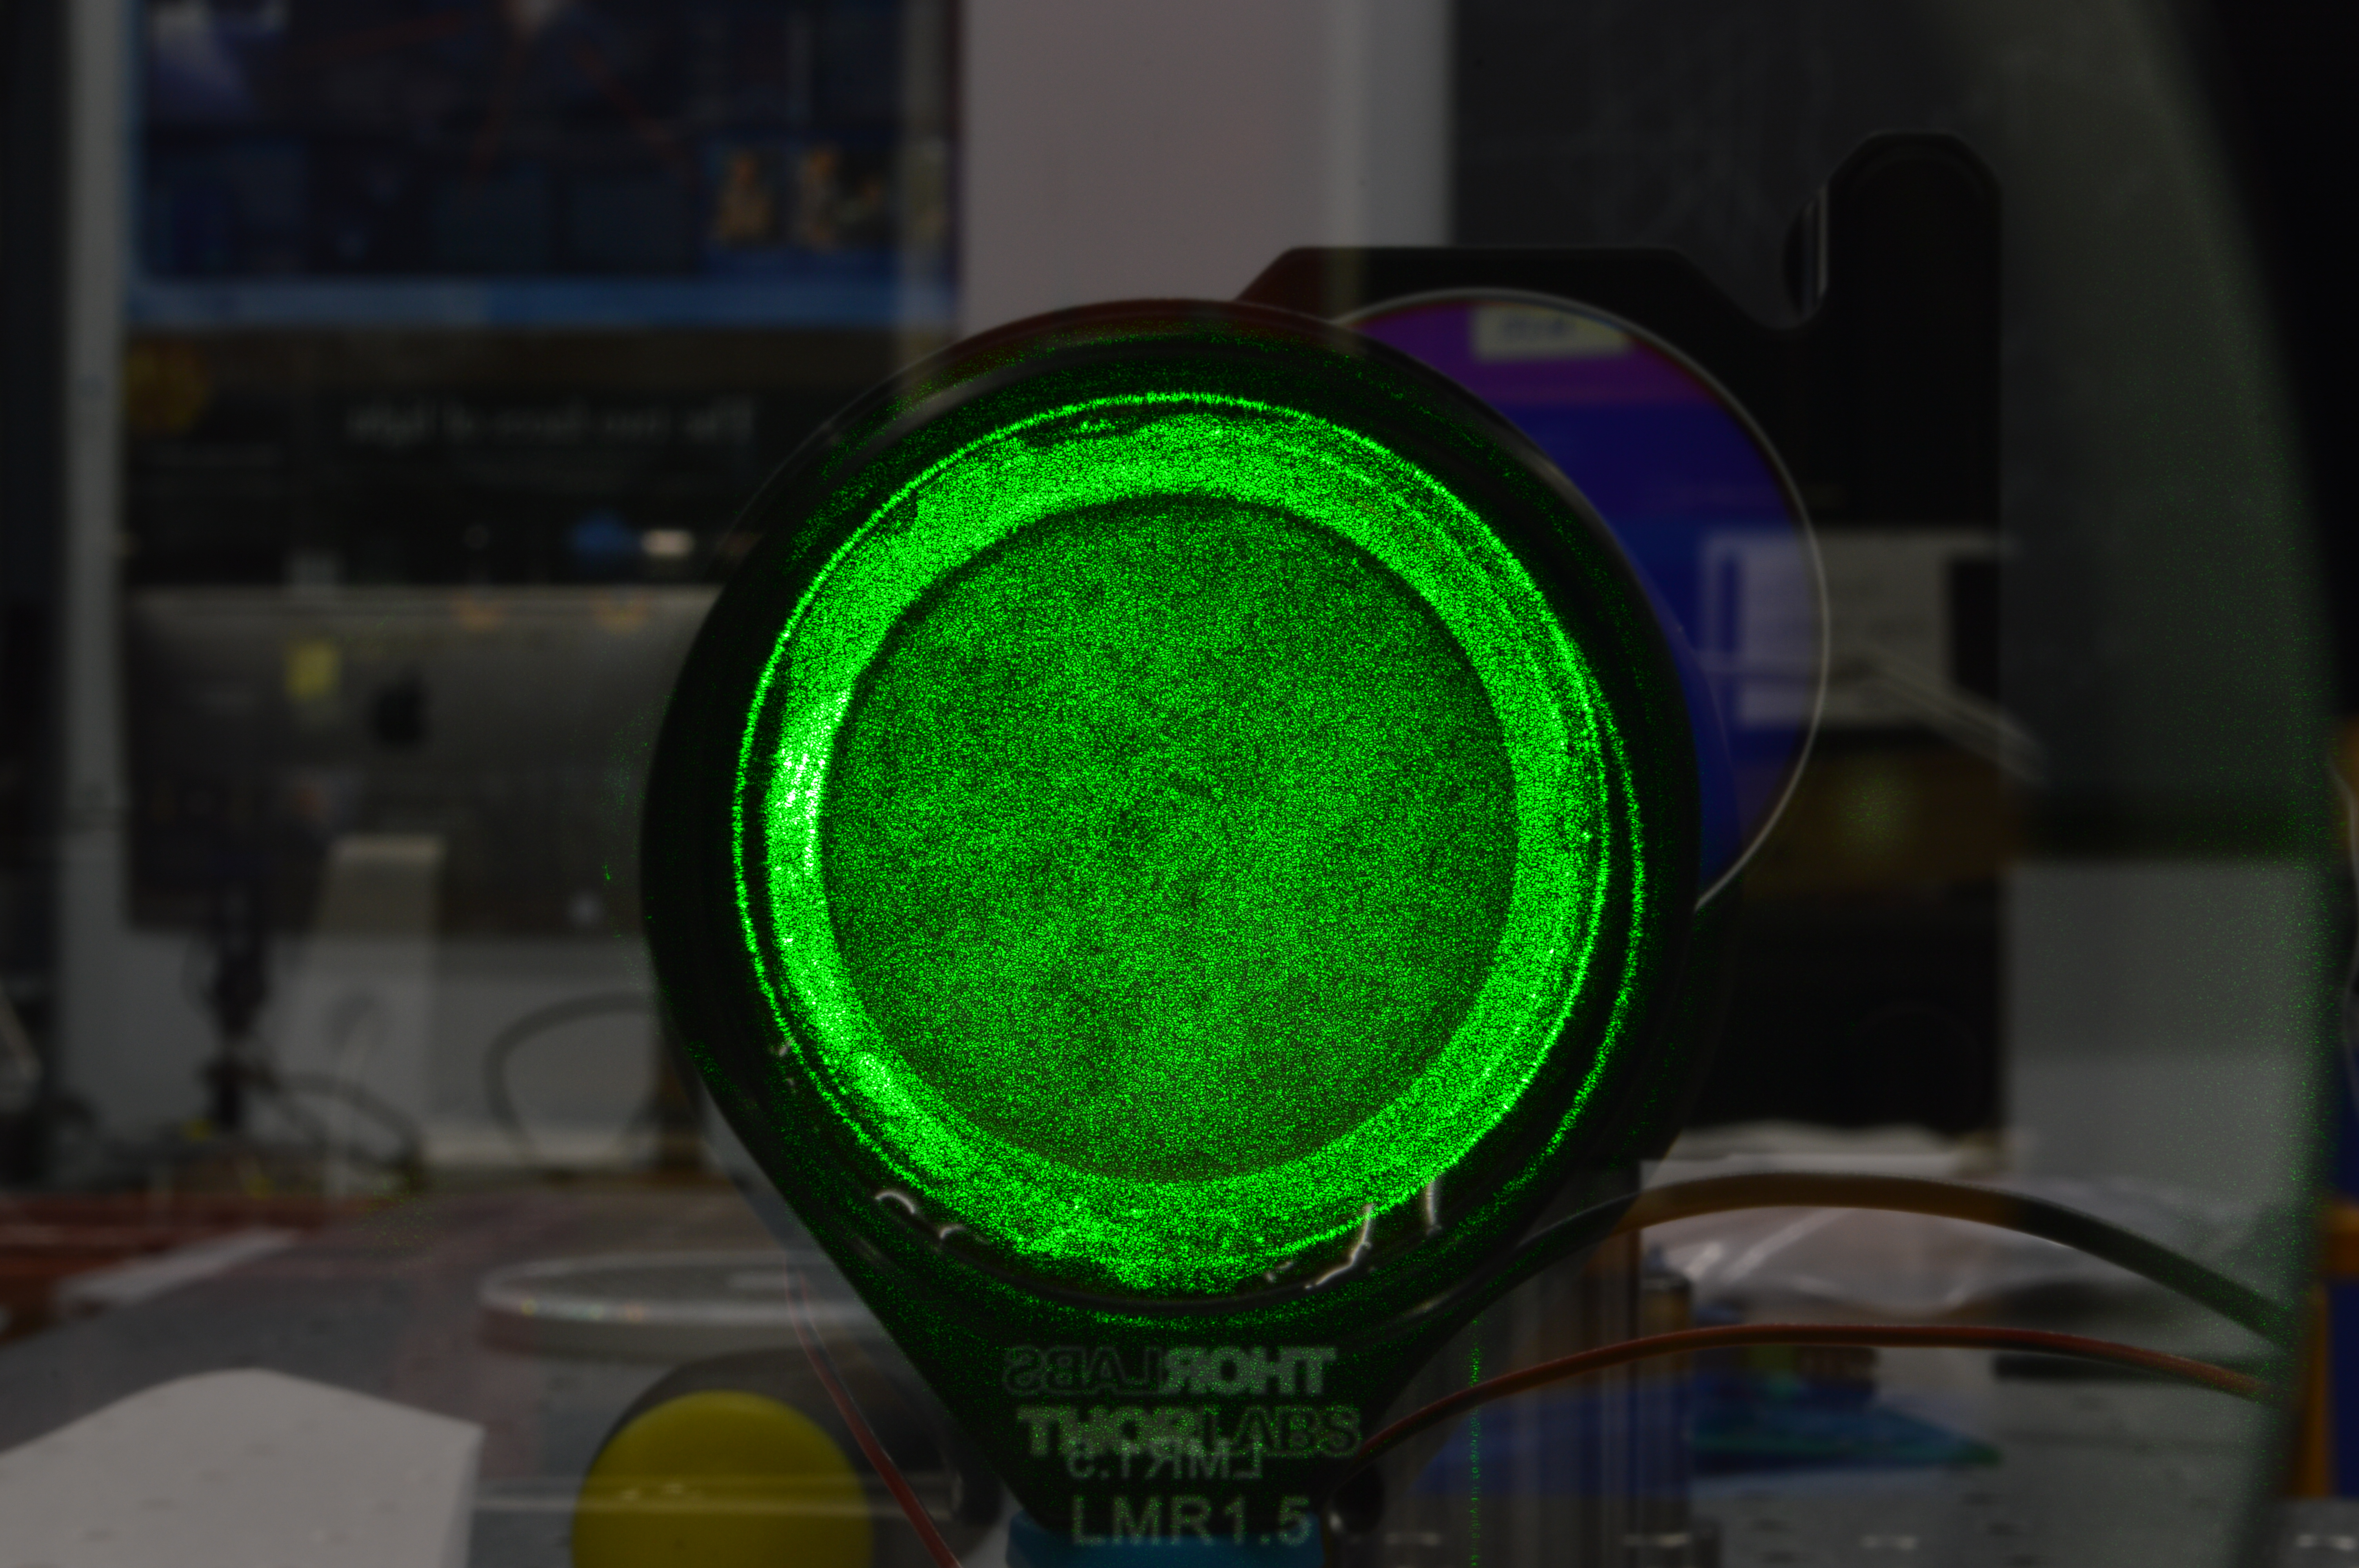
\includegraphics[width=.16\textwidth]{apertures/32.png}
% 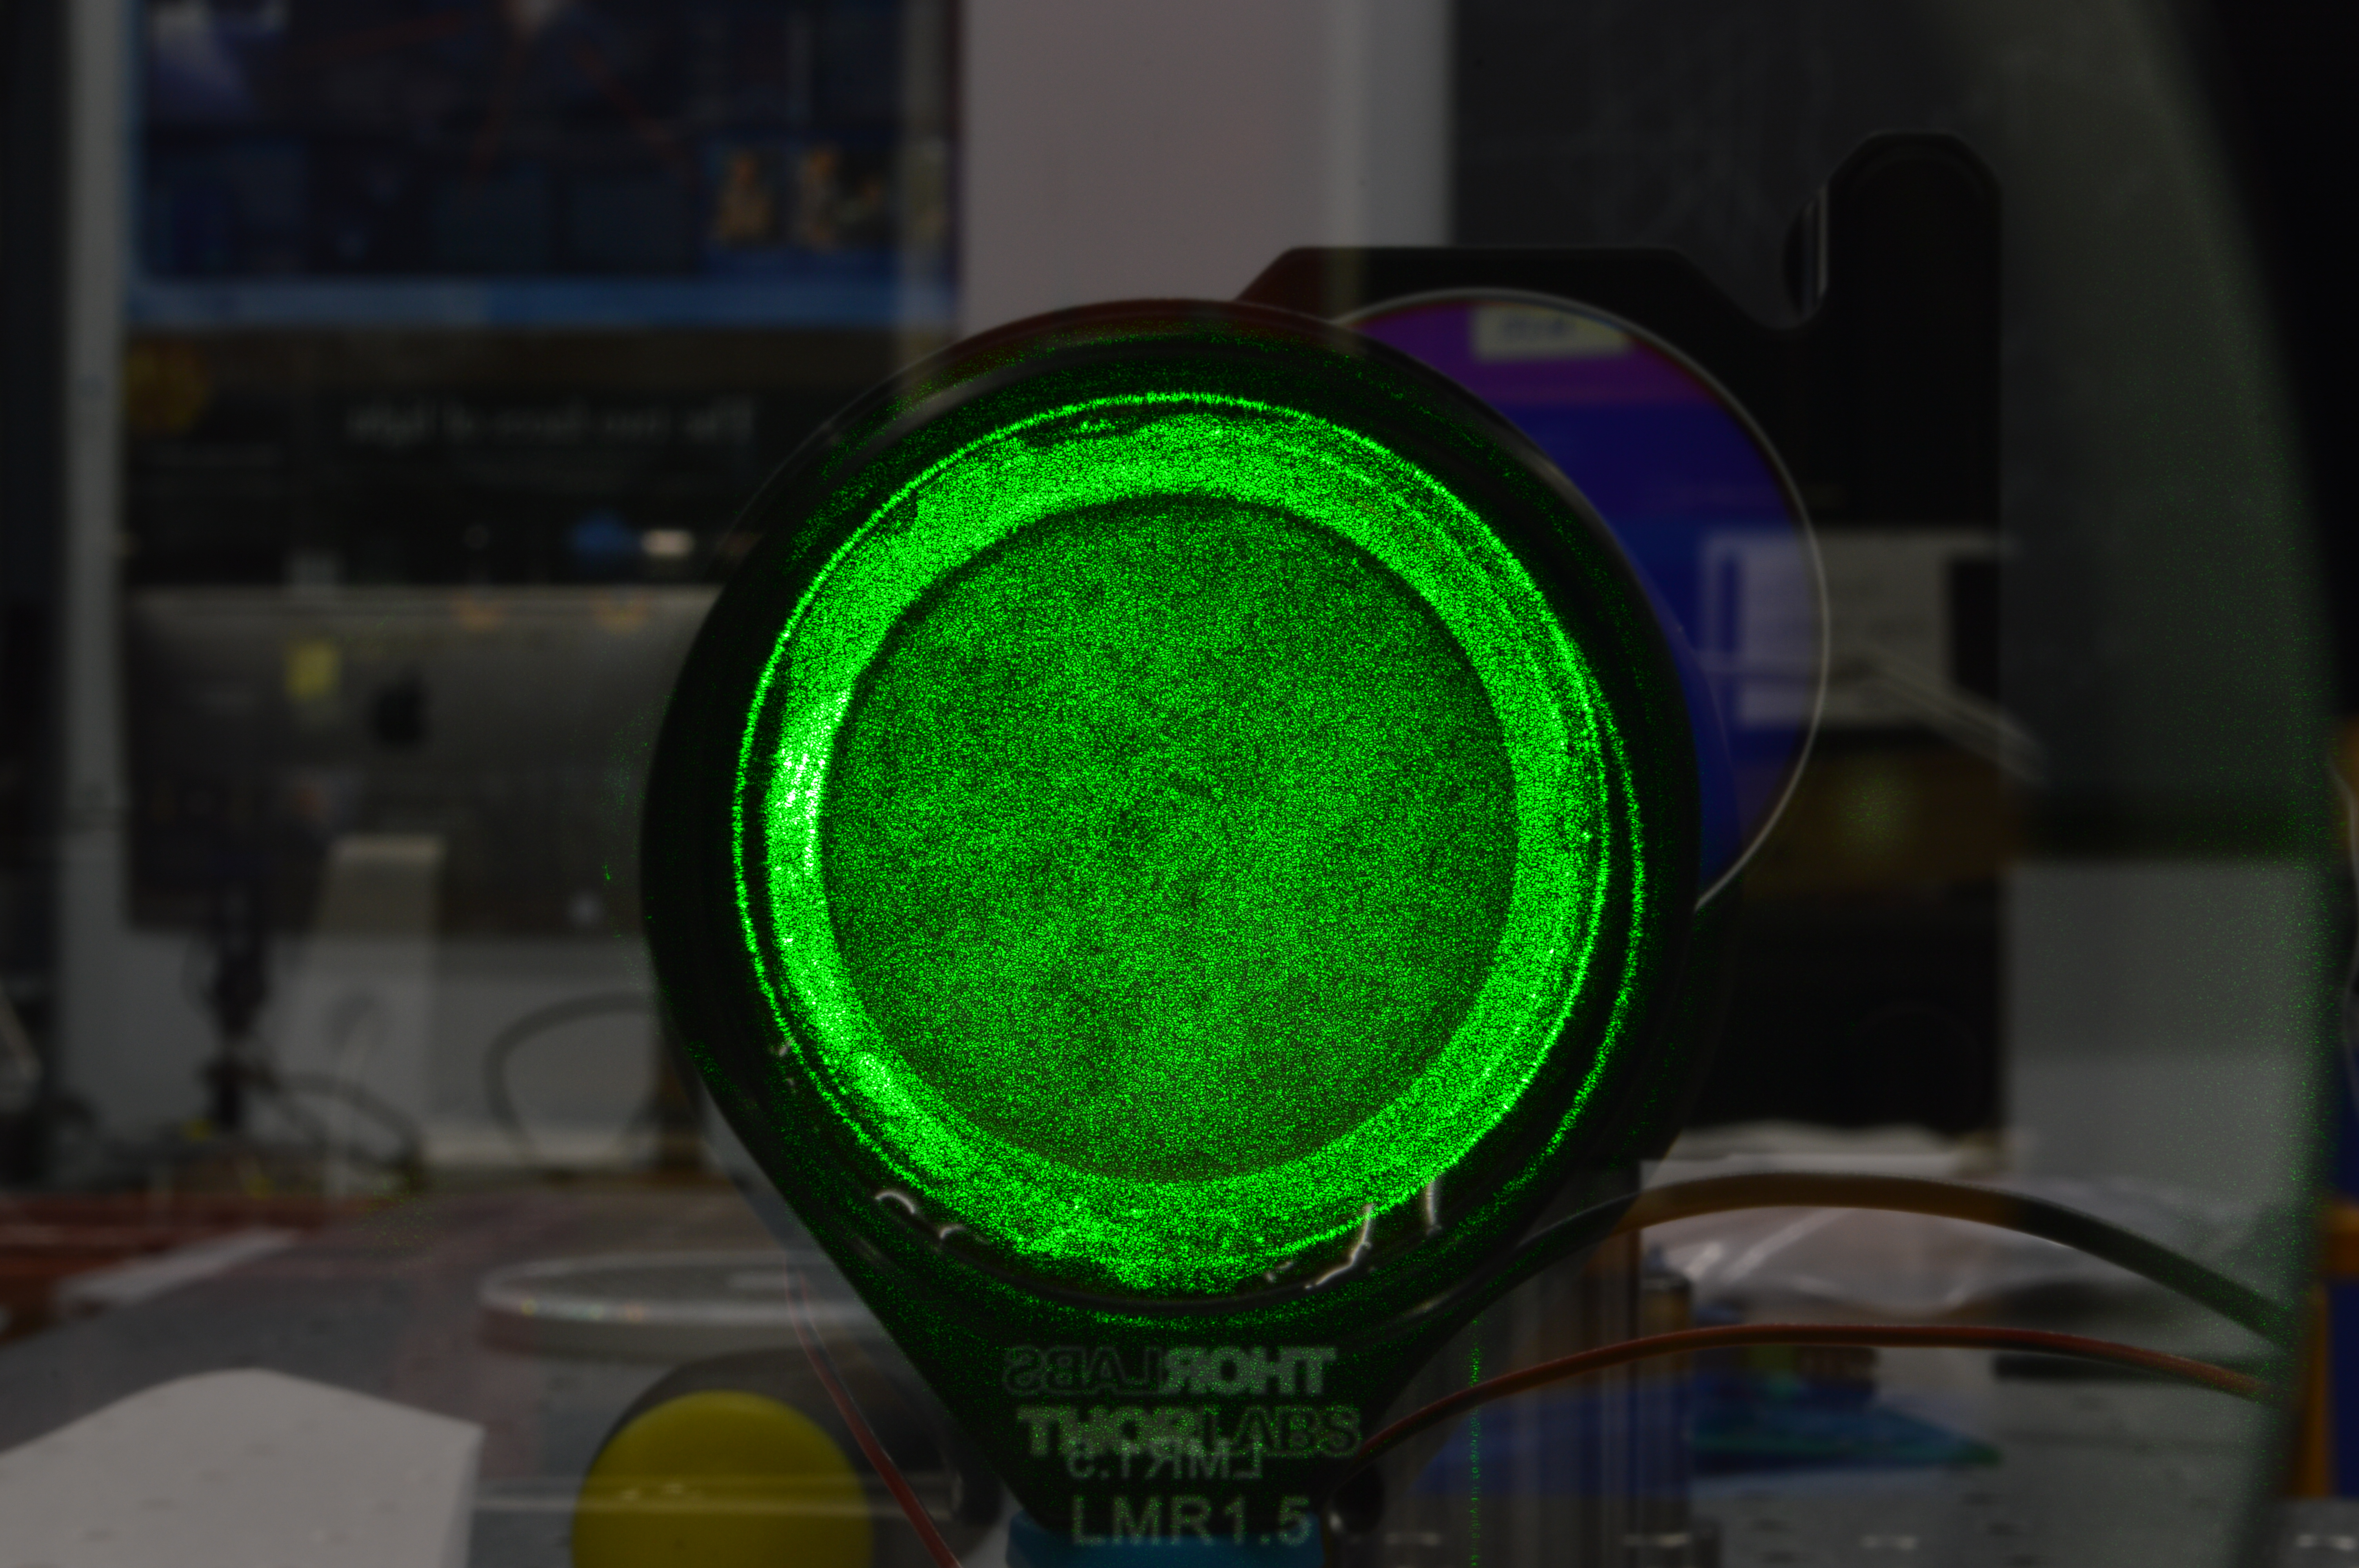
\includegraphics[width=.16\textwidth]{apertures/32.png}
% \end{center}

% \begin{center}
% {\bf Plot of amplitude vs voltage}
% (for an arbitrary pixel)
% \includegraphics[width=\textwidth]{cosine_check.png}
% \end{center}

% By varying voltages at a fixed rate with our function generator, and taking pictures of the speckles at fixed intervals using the ``burst mode'' of our camera, we were able to record how the amplitude of each pixel responds to offsets in the reference object.

% Note that these points were sampled at $x = 0, \frac{2\pi}{3}, \frac{4\pi}{3},...$, which is necesary to calculate the absolute phase.
\end{frame}

\begin{frame}{Calculating Relative Phases}
We took photos of speckle patterns for the following:
\begin{itemize}
	\item piezo at 0V, varying the voltate of the reference
	\item piezo at $\frac12$V, varying the voltate of the reference
\end{itemize}
By running the absolute phase calculations for both sets of images, we were able to get phases for each pixel of each set.

\vspace{0.5cm}
Taking the differences of the absolute phases gives us a relative phase for each pixel of the image. This corresponds to how much each point on the piezo has shifted.
\end{frame}

\section{Results}
\begin{frame}{Results}

\end{frame}

\section{Conclusions}
\begin{frame}{Conclusions}

\end{frame}

\section{Future Research}
\begin{frame}{Future Research}
Some additional directions in which this could be taken include:
\begin{itemize}
\item{Visualizing the behavior of membrane oscillations, by computing the relative phase differences of the surface at several moments during the oscillation.}
\item{Analyzing the stress that can be handled by a material. This could be done by applying a force, looking at the phase shifts, and looking for discontinuities that would imply cracking.}
\item{The approach itself could be improved by using more sophisticated cosine fitting algorithms to reduce the error from fitting a cosine to three points.}
\end{itemize}
\end{frame}

\section{References}
\begin{frame}{References}

\end{frame}
\end{document}